\documentclass[10pt,twocolumn]{article}
	
\usepackage{myfontstyle}
\usepackage{mypackages}
\usepackage{mymacros}
\usepackage{mycommands}
\usepackage{url}
\usepackage{textgreek}


\begin{document}
\thispagestyle{fancy1}

%%% Title and Abstract------------------------
\twocolumn[
\begin{center}
	\hrule
	\vspace{3pt}
	% Title:
	{\sffamily\bfseries\Large
		Report for Laboratory Four: RLC Frequency Response 
	} \\
	{\color{gray}
		\vspace{3pt}
		\hrule
		\vspace{3pt}
	}
	{
		\hspace*{\fill}
		Austin Piper
		\hspace*{\fill}
		Alex Blakely
		\hspace*{\fill}
		Irfan Ahmed
		\hspace*{\fill}
%		Fourth Author    % uncomment these two lines if there's a fourth author
%		\hspace*{\fill}
	}\\
	\vspace{3pt}
	{\itshape
		\hspace*{\fill}
		Department of Mechanical Engineering, Saint Martin's University
		\hspace*{\fill} \\
		\hspace*{\fill}
		ME/EE 316---Mechatronics \& Measurements Laboratory
		\hspace*{\fill}
	}\\
	\vspace{3pt}
	{
		\hspace*{\fill}
		\today{} % today's date ... can type manually instead
		\hspace*{\fill}
	}
	\vspace{3pt}
	{\color{gray}\hrule}
%	\vspace{2pt}
\end{center}
% Abstract:
\begin{adjustwidth}{1.5in}{1.5in}
{\small
\noindent\textbf{Abstract.} \hspace{1em}
	In this lab exercise, we measured the steady-state response of the output voltage of an RLC circuit with a sinusoidal voltage source. We recorded the data by hand, and used MATLAB to plot the data and derive a model. Finally, we compared the analytic model to the experimental data.
}
\end{adjustwidth}
\vspace{9pt}
\hrule
\vspace{1\baselineskip}
]

%%% Body -------------------------


\section{Introduction} 
\label{sec:introduction}

An RLC circuit is a circuit that contains a resistor, and inductor, and a capacitor. This class of circuits is often used as oscillators. The characteristics of this type of circuit make it useful in signal filtering.

While, by definition, this kind of circuit can be any combination of these three circuit elements, in this experiment we put them together in Series. As \autoref{fig:diagram} shows, we assume that the voltage source (a signal generator) has a resistance Rs (which has a value of 50 \Omega).

In this lab, we observed both the input signal and the output signal of this circuit (as defined in the aforementioned diagram). In addition to witnessing the actual effects in terms of amplitude and phase shift, the theoretical shift and amplitude ratios were also considered.

\begin{figure}[bt]
	\centering
	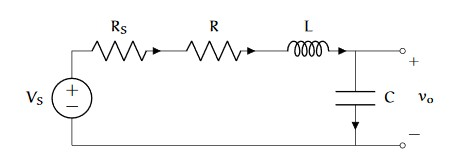
\includegraphics[width=.9\linewidth]{figures/RLCDiagram.JPG}
	\caption{The RLC Circuit}
	\label{fig:diagram}
\end{figure}

\section{Materials and Methods}

\begin{enumerate}
\item 
1 LabVIEW and MATLAB compatible device 
\item 
1 myRIO microcontroller
\item
1 breadboard
\item
1 BNC Y- or T-connector
\item
2 BNC-to-allifator cables
\item
4 male jumper wires
\item
78 ohm resistor
\item
100mH inductor
\item
700 pF capacitor
\item
multimeter
\item
oscilloscope
\item
function generator
\end{enumerate}

The RLC circuit (figures 1 and 2) was built after measuring both the resistance of the resistor (noting that the internal resistance of the function generator was fifty ohms) and the capacitance of the capacitor. After its construction, jumpers were inserted to measure both the input voltage of the function generator and the output voltage using the LabVIEW software. After setting the function generator to a sinusoidal input at 1000 Hz (1kHz), we began making our recordings of the data including the phase shift and output voltage. We went from 1 kHz to 50,000 kHz intermittently in order to see how the amplitudes and phase shifts viewed on the oscilloscope were affected by different frequencies along the way. After each different frequency setting it was important to view both the input and output sinusoids so that any patterns could be taken note of.  


\section{Results}
\label{sec:results}

\begin{figure}[bt]
	\centering
	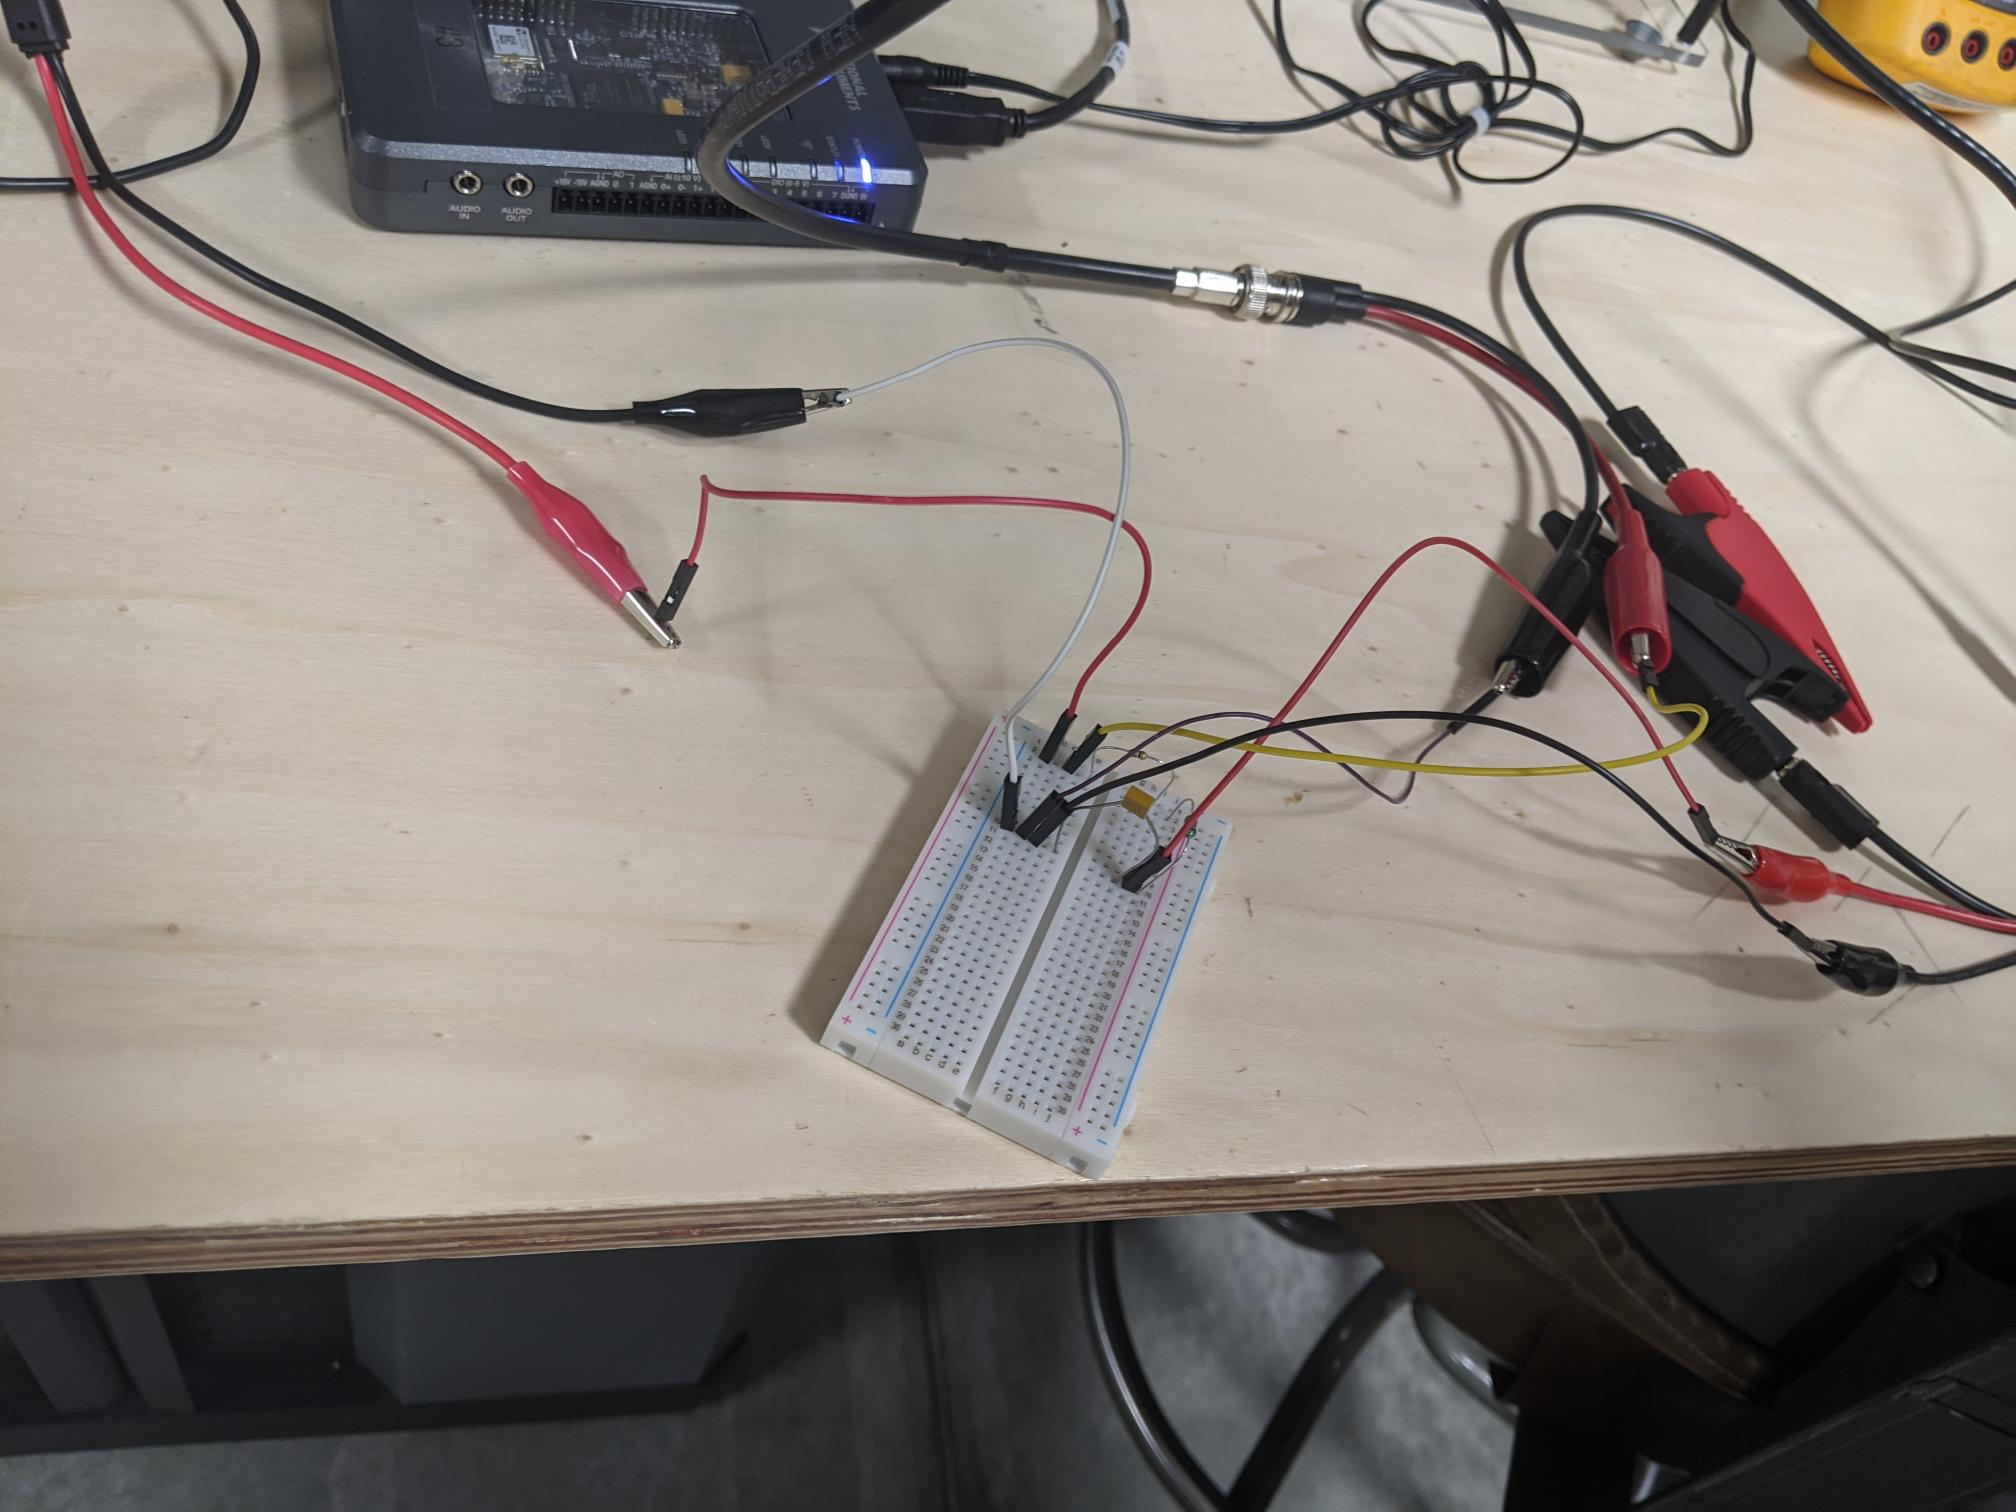
\includegraphics[width=.9\linewidth]{figures/RLCcircuit.PNG}
	\caption{Our RLC Circuit}
	\label{fig:diagram2}
\end{figure}

This lab produced four different data streams that were recorded by our group: the actual frequencies of the sinusoidal outputs and inputs, the peak-to-peak amplitudes of the of the input and output voltages, and the time lags between them. Using these data streams and the recorded phase shifts of each of the frequencies we were able to view when the expected resonance occurred and the time lags decreasing from the starting 1 kHz to our ultimate 50000 kHz. Our data showed the physical manifestation of resonance in terms of sinusoidal output and input waves, where they continually become more and more out of phase with one another due to the capacitor and inductor’s relationship to one another until a certain frequency is reached, where they cancel each other out in a sense, and the phase is back in line with its original sinusoid. We saw this occurrence at about 600 kHz. This also agreed with our Amplitude ratio graph \autoref{fig:rvsF}, showing our natural frequency to be at approximately 625 kHz.

\section{Discussion}

A common real-world example of a circuit’s transient response leading to a steady state is the flip of a light switch. A sudden input of voltage will take some amount of time for the steady state of the circuit to be reached and this is what we see with our RLC circuit in this lab. As we applied increasingly large frequencies to the circuit, we witnessed phase shift of the sinusoids increase up to 90 degrees as we approached 600 kHz as the output voltage decreased in kind \autoref{fig:phivsF}. For a series circuit at what is known as resonance, both the capacitance and inductive reactance would be equal, meaning that the phase angle (phase shift) would be at zero. 

\begin{figure}[bt]
	\centering
	\includegraphics[width=.9\linewidth]{figures/rvsF.png}
	\caption{r vs Frequency}
	\label{fig:rvsF}
\end{figure}

\begin{figure}[bt]
	\centering
	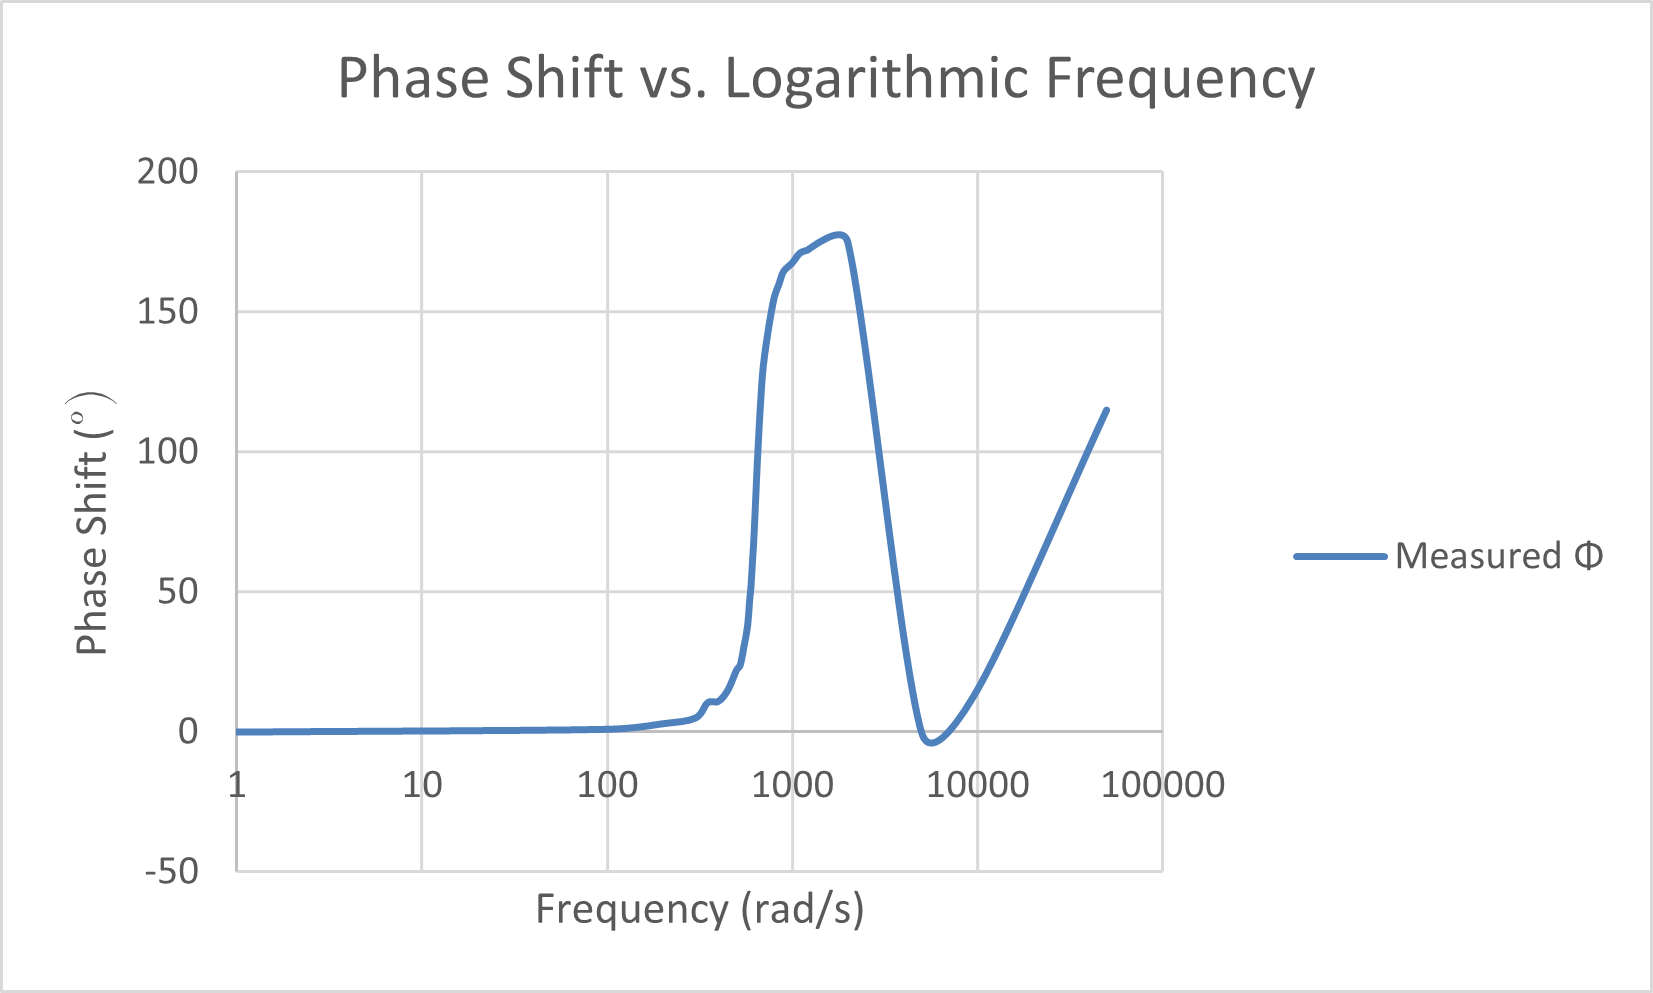
\includegraphics[width=.9\linewidth]{figures/phivsF.png}
	\caption{\Phi vs Frequency}
	\label{fig:phivsF}
\end{figure}

\begin{figure}[bt]
	\centering
	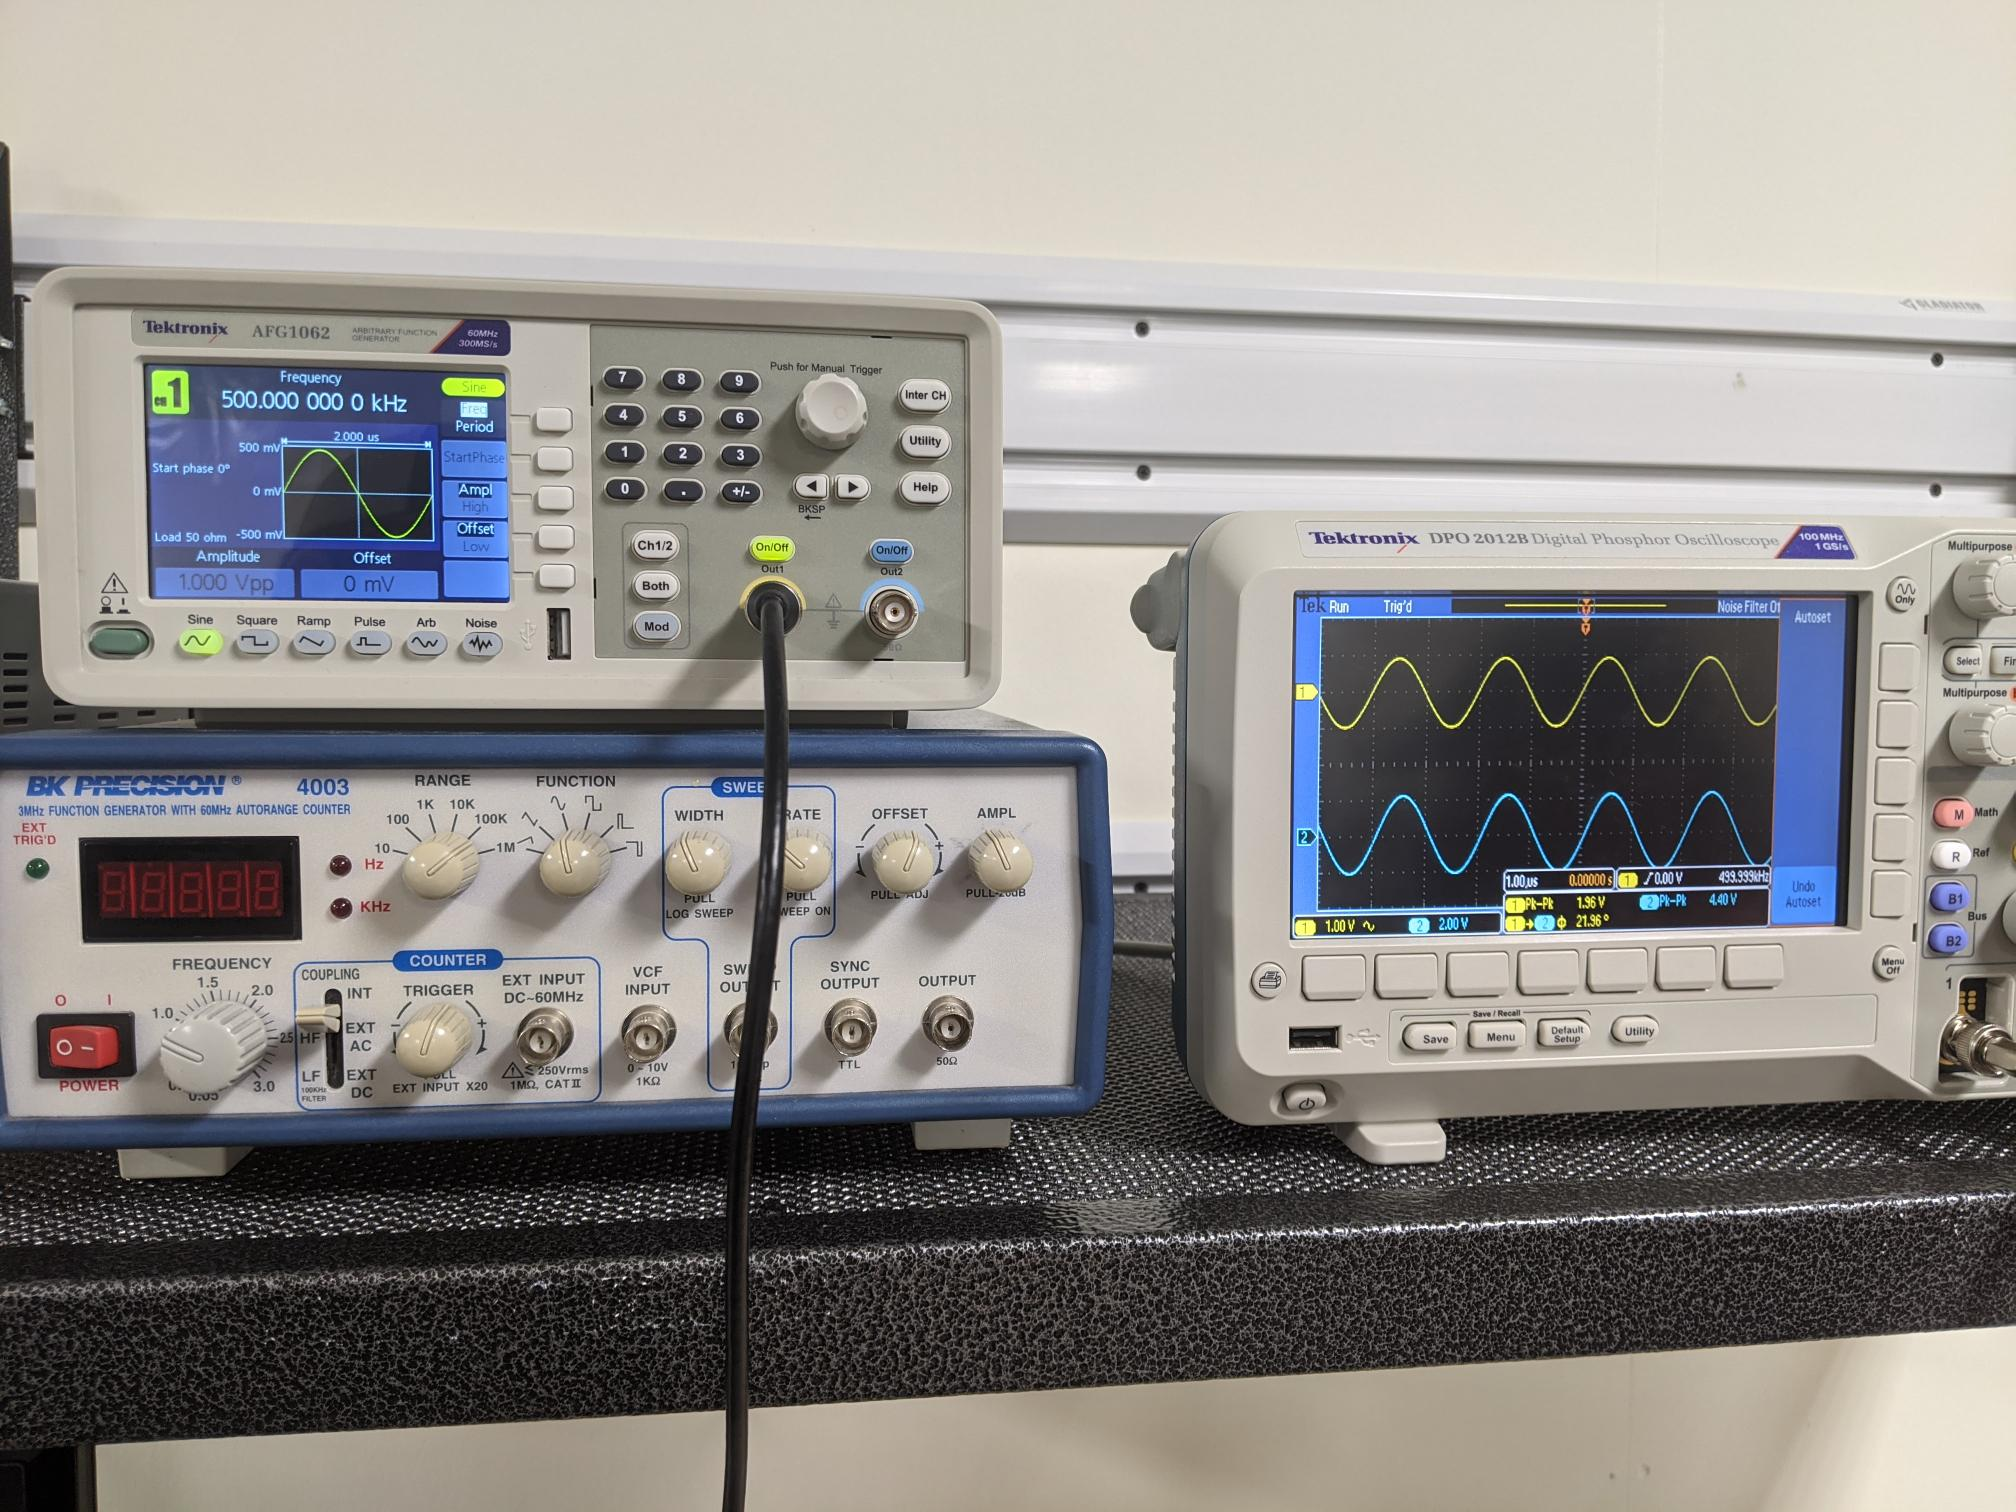
\includegraphics[width=.9\linewidth]{figures/img1.png}
	\caption{Function generator and Oscilliscope at 500kHz}
	\label{fig:500kHz}
\end{figure}

\begin{figure}[bt]
	\centering
	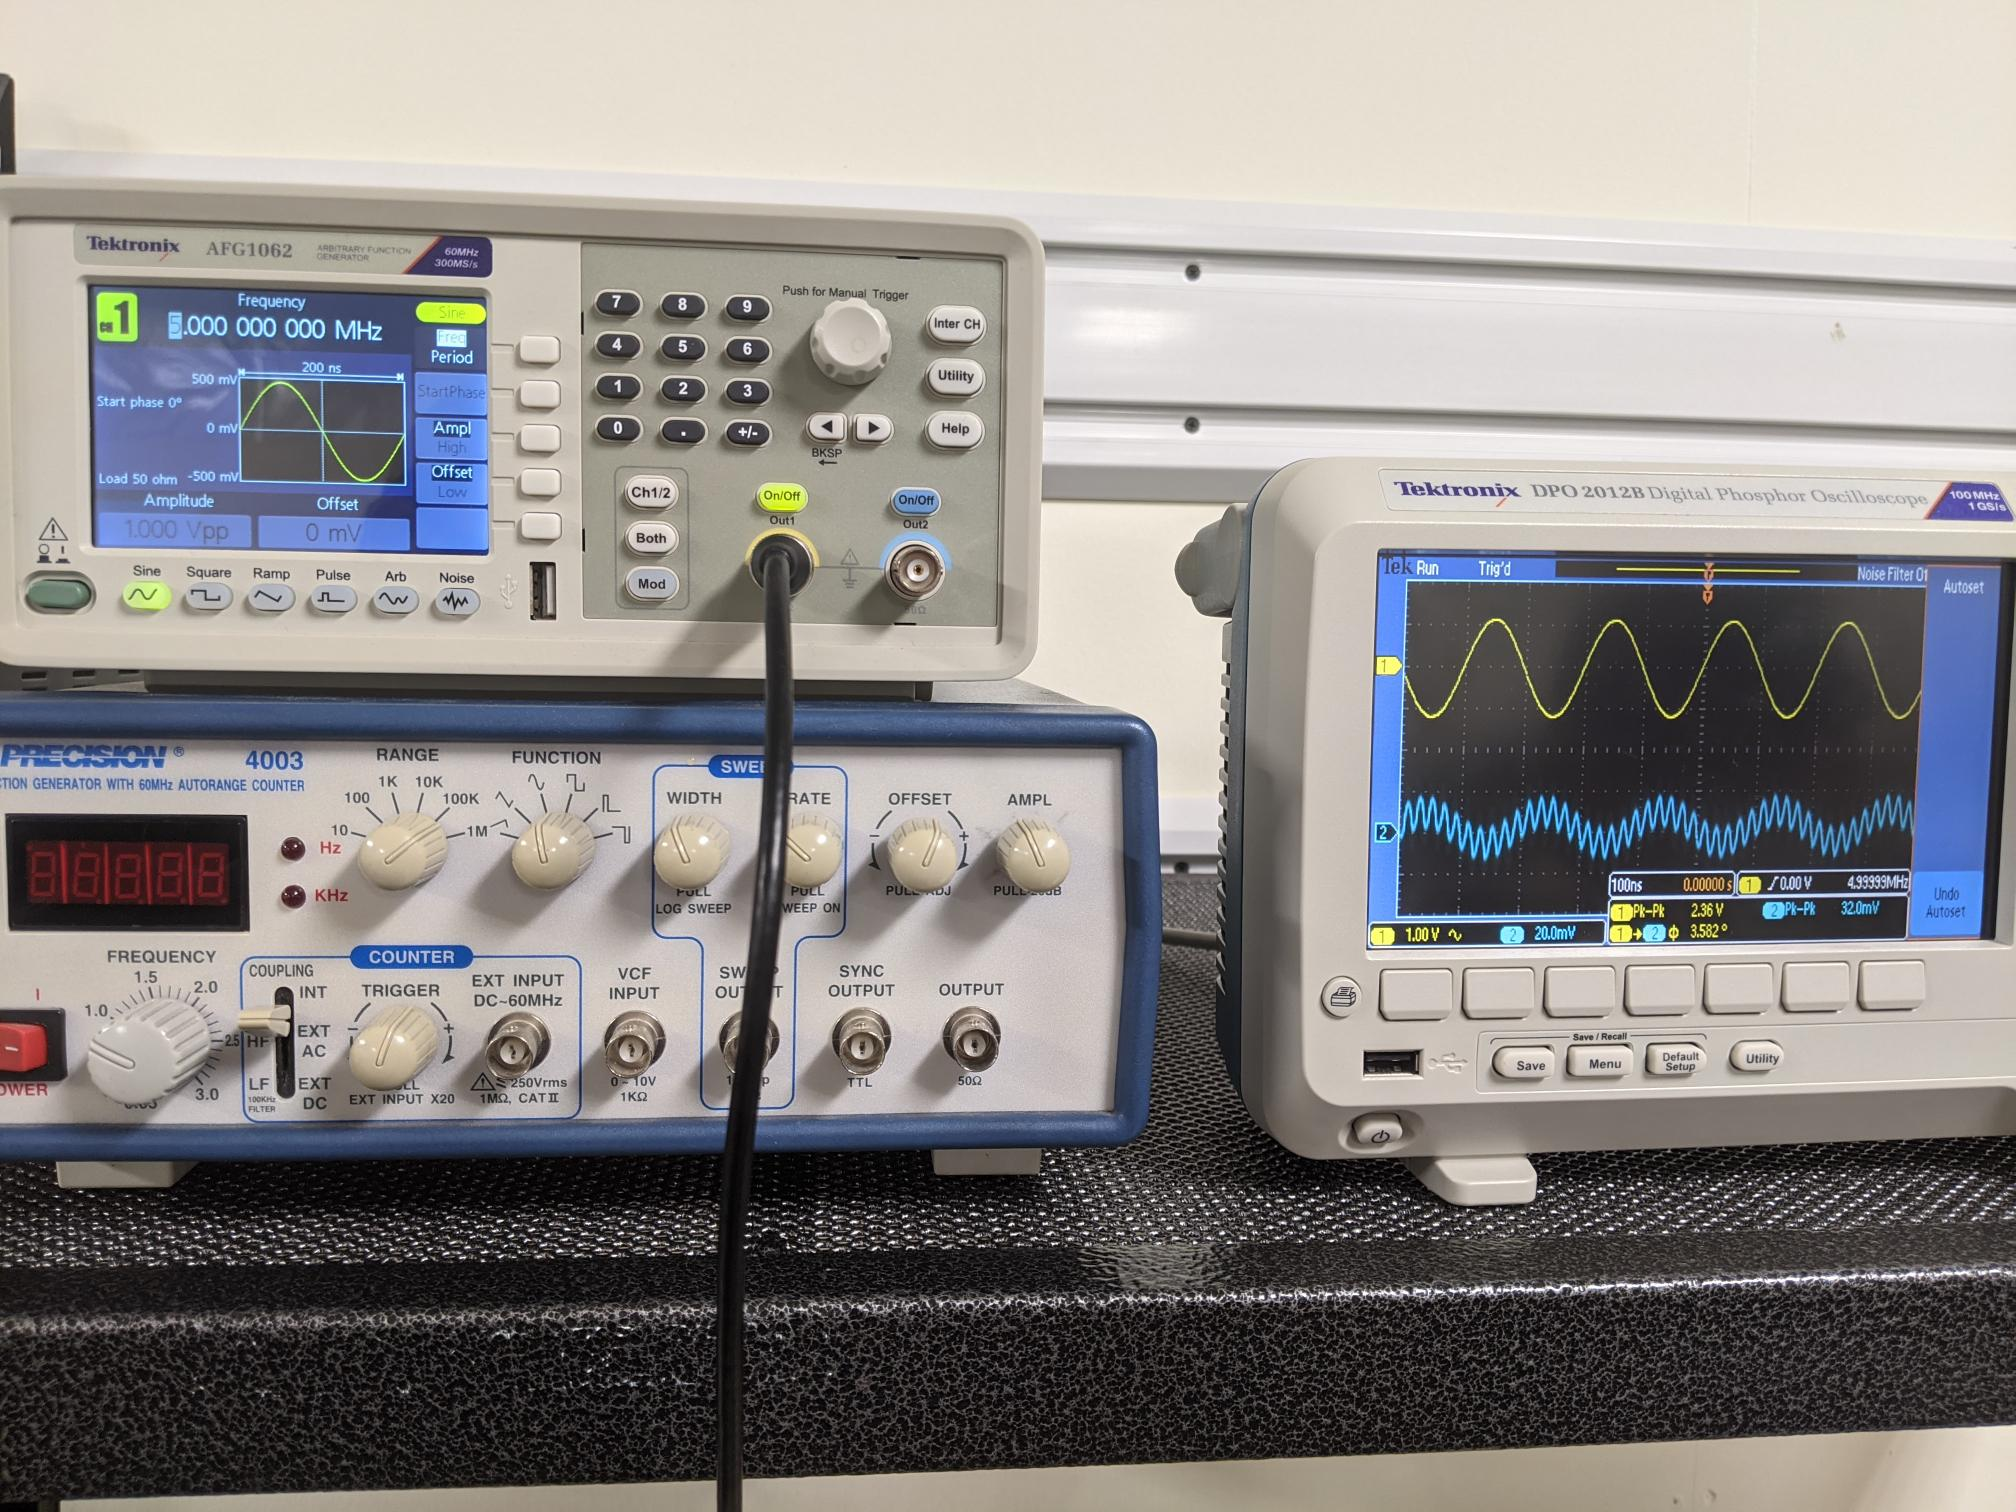
\includegraphics[width=.9\linewidth]{figures/img2.png}
	\caption{Function generator and Ocilliscope at 5MHz}
	\label{fig:5MHz}
\end{figure}
\section{Author Contributions}

Irfan wrote the abstract and the introduction, and also added the circuit diagram. Alex wrote the materials and methods, the discussion, and part of the results. Austin worked on the results and calculations. We all checked the calculations, and checked over the report for final edits.

\section{Equations}

Once completing a circuit analysis we found our amplitude ratio equation as well as out Phase shift equation.
\begin{align*}
	
	 r(\omega) &= |\frac{1}{\sqrt{\left(1 - \omega^2*L*C\right)^2 + j*\omega^2*C^2\left(R_{s}+R\right)^2}}|
	 
	 \Phi(\omega) = tan^-1(\frac{\omega*C*\left(R_{s}+R\right)}{1-\omega^2*L*C})
\end{align*}

\begin{table}[bt]
	\begin{tabularx}{1\linewidth}{ lXX }
		\hline
		 & \textbf{R (Ω)} & \textbf{C (pF)} \\
		\hline
		nominal & $78$ & $700$ \\
		measured & $66.78$ & $690$ \\
		\hline
	\end{tabularx}
	\caption{Multimeter Measurements}
	\label{tab:Tab1}
\end{table}

\begin{table}
	\begin{tabularx}{1\linewidth}{ lXXXX|cXXXXXXXXXXXXXXXXXXXXXXXXXXXXX }
		\hline
		 & \textbf{Freq.(kHz)} & \textbf{Vs-Vrs (V)} & \textbf{Vo (V)} & \textbf{Phase Shift   (degrees)}\\
		\hline
		& 1 & 2.16 & 2.12 & 0 \\
	 
		\cline{1-5}
		& 100 & 2.16 & 2.16 & 1 \\
	
		\cline{1-5}
		& 200 & 2.16 & 2.32 & 3 \\
		
		\cline{1-5}
		& 300 & 2.16 & 2.66 & 5 \\
		
		\cline{1-5}
		& 350 & 2.10 & 2.90 & 10.5 \\
		
		\cline{1-5}
		& 400 & 2.09 & 3.24 & 11 \\
		
		\cline{1-5}
		& 450 & 2.04 & 3.76 & 15\\
		
		\cline{1-5}
		& 500 & 1.96 & 4.48 & 22 \\
	
		\cline{1-5}
		& 525 & 1.90 & 4.92 & 24 \\
		
		\cline{1-5}
		& 550 & 1.74 & 5.40 & 30.6 \\
		
		\cline{1-5}
		& 575 & 1.61 & 5.85 & 38 \\
		
		\cline{1-5}
		& 590 & 1.50 & 6.16 & 47 \\
		
		\cline{1-5}
		& 600 & 1.44 & 6.28 & 52 \\
		
		\cline{1-5}
		& 610 & 1.38 & 6.36 & 60 \\
	
		\cline{1-5}
		& 625 & 1.30 & 6.44 & 72 \\
		
		\cline{1-5}
		& 650 & 1.26  & 6.20 & 97 \\		
		\cline{1-5}
		& 675 & 1.34 & 5.80 & 117 \\
		
		\cline{1-5}
		& 700 & 1.47 & 5.20 & 131 \\
		
		\cline{1-5}
		& 750 & 1.69 & 4.00 & 145 \\
		
		\cline{1-5}
		& 800 & 1.86 & 3.06 & 155 \\
	
		\cline{1-5}
		& 850 & 1.92 & 2.42 & 160 \\
		
		\cline{1-5}
		& 900 & 2.00 & 1.98 & 164.5 \\
		
		\cline{1-5}
		& 1000 & 2.06 & 1.4 & 167.5 \\
		
		\cline{1-5}
		& 1100 & 2.10 & 1.06 & 171 \\
		
		\cline{1-5}
		& 1200 & 2.10 & 0.84 & 172 \\
		
		\cline{1-5}
		& 2000 & 2.16 & 0.23 & 175 \\
		
		\cline{1-5}
		& 5000 & 2.40 & 0.034 & 0 \\
		
		\cline{1-5}
		& 10000 & 3.44 & 0.05 & 15 \\
		
		\cline{1-5}
		& 50000 & 0.88 & 0.038 & 115 \\
		
		\cline{1-5}
		
		\hline
	\end{tabularx}
	\caption{Captured Data}
	\label{tab:Tab2}
\end{table}

\end{document}  
